\section{Results - Scale Testing}
\label{ResultsScaleTesting}
%
The dataset contains several zero-answers which, due to a programming error, could happen when subjects did not answer on a scale. Two criteria were used to determine when to exclude some of the zero-points that occurred because of a non-answered scale. 1) If all scale ratings presented on one of the pages are zero, it was probably because subjects skipped a page and 2) If there is a strong tendency for high ratings on a scale and a single zero-answer seems unlikely, it was denoted as a missing answer.\\

\noindent
The different ratings on the scales in the second test are visualised on \autoref{fig:Boxplot}.
%
%\begin{figure}[H]
%	\centering
%	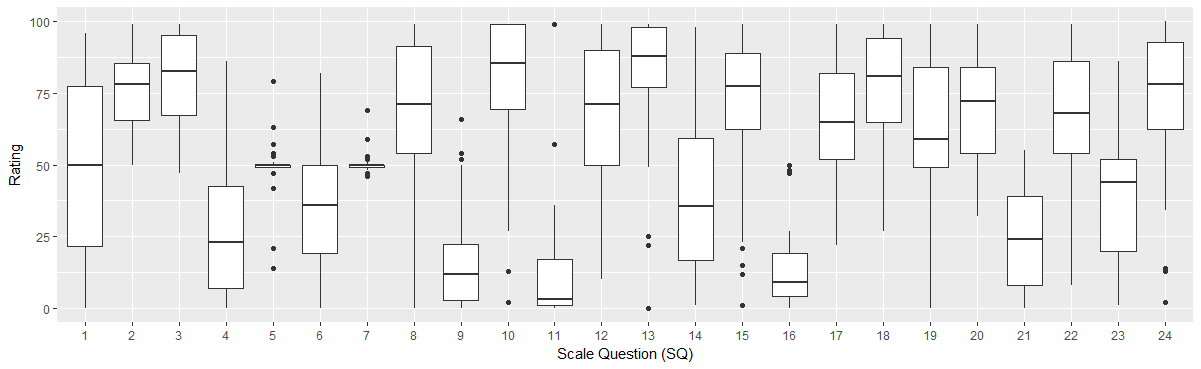
\includegraphics[width = 0.49\textwidth]{Figure/Boksplot24uden0}
%	\setlength\abovecaptionskip{-1.2\baselineskip} 
%	\caption{Boxplot showing the 24 attributes. The boxplot shows the median, where the box is ranging from 25-75 \% of the data, and the whiskers from 0-25 \% and 25-100 \% of the data.}
%	\label{fig:Boxplot}
%\end{figure}
%\noindent
%

\begin{figure*}[!b]
	\centering
	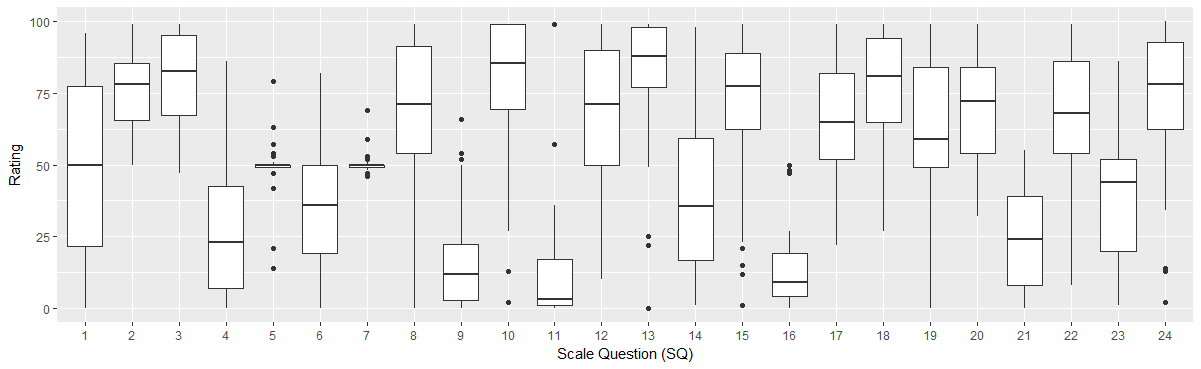
\includegraphics[width=6.9in]{Figure/Boksplot24uden0}
	\label{fig:Boxplot}
%	\hfil
%	\subfloat[]{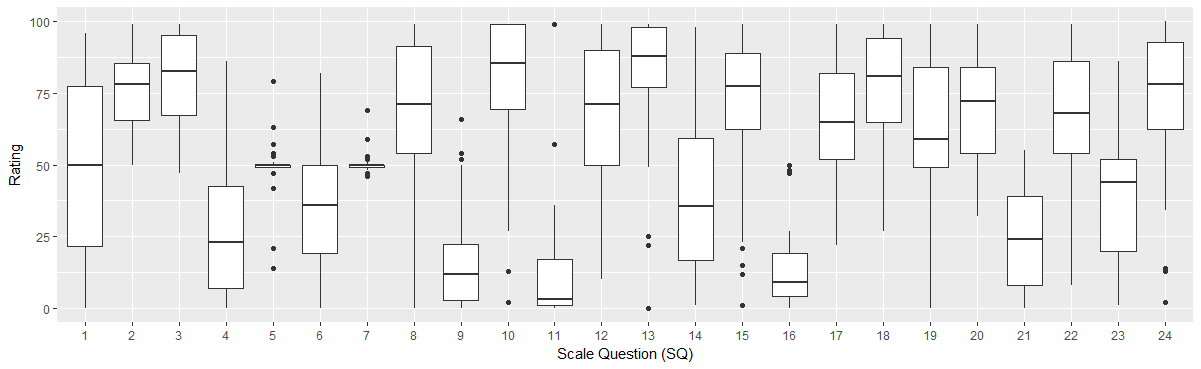
\includegraphics[width=2.5in]{Figure/Boksplot24uden0}
%		\label{fig_second_case}}
	\caption{Boxplot showing the 24 attributes. The boxplot shows the median, where the box is ranging from 25-75 \% of the data, and the whiskers from 0-25 \% and 25-100 \% of the data.}
\end{figure*}

%
From \autoref{fig:Boxplot}\fxnote{Ifølge Dorte kunne vi sagtens gøre brug af farver her til at gruppere boksplottet. Jeg r enig! (fx. 1,4, 8, 12, 14, 19 er én farve, da de beskriver boxplots med stor variation osv.)... undskyld, Juliane.} it is notable that their exists much greater variation in some scales compared to others. For some SQs, a big part of the scale is used (1, 4, 8, 12, 14, 19), where for others a smaller part of the scale is used (2, 3, 5, 7, 9, 11, 13, 16). Furthermore some of the scale ratings appears normal distributed (1, 2, 6, 17, 20, 21) and others appears skewed (8, 9, 10, 11, 13, 18). In some SQs the data accumulates around midpoints or terminal points (5, 7, 9, 10, 11, 13). SQ5 and SQ7 are centralised around the midpoint, which can relate to the label (fine) being too broadly describing. \\ 

\noindent
When looking at gender differences SQ21 seem to reveal a difference. Females rate SQ21 twice as high as males, which also seems to apply to SQ4 and SQ11. It suggests that they experience the robot's movements more calm compared to males, but also that they find the robot less intrusive and startling.\\

\noindent
When conducting a PCA on all the scale results it shows that only 80 \% of the total variance is explained when using 7 dimensions, which is why PCA relating to different groups as the robot's height, distance and direction is conducted in order to reduce the dimensions and be able to explain more of the variance. \autoref{fig:Scree} shows a scree plot from PCA relating to the robot's height, where 94.1 \% of the variance is explained when using three dimensions. \autoref{fig:biplot} shows the biplot relating to the robot's height. Similar biplots were made for direction and distance. The results were:

\noindent
\textbullet \textbf{Height:} SQ19 appears to contribute the most to PC1. SQ1 the most to PC2. \\
\textbullet \textbf{Distance:} SQ1 appears to contribute the most to PC1 along with SQ15. SQ10 contributes most to PC2.\\
\textbullet \textbf{Direction:} SQ10 contributes most to PC1. SQ22 and SQ23 contributes almost equally much to PC2.\\
%
\begin{figure}
	\centering
	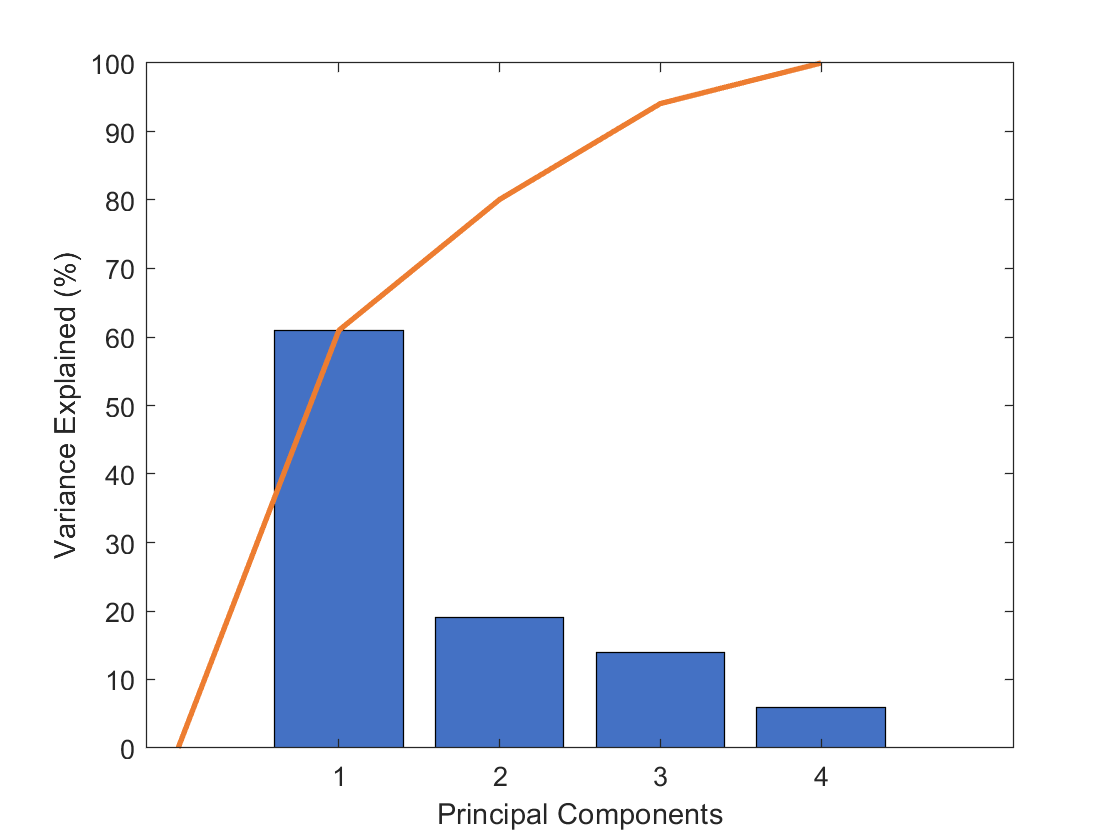
\includegraphics[width = 0.40\textwidth]{Figure/Scree.png}
	\setlength\abovecaptionskip{-0.5\baselineskip} 
	\caption{Scree plot showing the connection between the number of Principal Components and Variance Explained [\%]: PC1 (61 \%), PC2 (19.1 \%), PC3(14 \%), PC4(5.9 \%).}
	\label{fig:Scree}
\end{figure}
\noindent

%
\begin{figure}
	\centering
	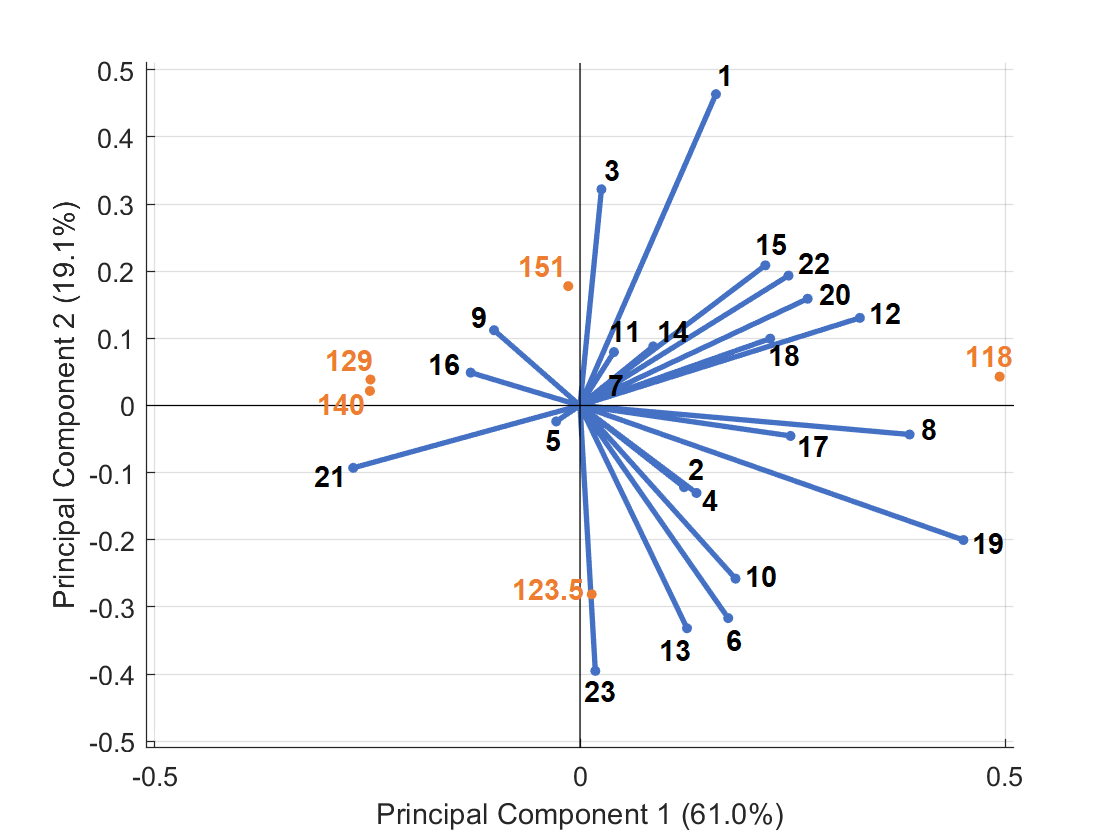
\includegraphics[width = 0.40\textwidth]{Figure/RHeight-Biplot.png}
	\setlength\abovecaptionskip{-0.5\baselineskip} 
	\caption{Biplot showing how the different attributes contributes to components and which attributes that correlates. The black numbers denotes SQ and the red to the different heights in cm.}
	\label{fig:biplot}
\end{figure}
\noindent
%
Furthermore 2D and 3D biplots from the different PCAs shows positive and negative correlations between attributes/scale questions. These correlations are presented in \autoref{tab:CorrelationsFromPCA}.
%
\begin{table}
	\centering
	\caption{Correlations from PCA}
	\label{tab:CorrelationsFromPCA} 
	\begin{tabular}{ c|c|c }
		\centering
		PCA & Positive correlation & Negative correlation \\ \hline
		\multirow{5}{*}{Height} & SQ08  + SQ17 & SQ02  + SQ09 \\
		& SQ10 + SQ13 & SQ04 + SQ12 \\
		& SQ12 + SQ18 & SQ12 + SQ21 \\
		& SQ14 + SQ15 & SQ16 + SQ19 \\
		& SQ20 + SQ22 & SQ18 + SQ21\\ \hline
		\multirow{6}{*}{Distance} & SQ01 + SQ12 & SQ02 + SQ09 \\
		& SQ07 + SQ17 & SQ05 + SQ21 \\
		& SQ08 + SQ21 & SQ10 + SQ13 \\
		& SQ10 + SQ22 & SQ13 + SQ22 \\
		&  & SQ14 + SQ16 \\	
		&  & SQ19 + SQ20 \\ \hline	
		\multirow{5}{*}{Direction} 
		& SQ05 + SQ07 & SQ01 + SQ12 \\
		& SQ08 + SQ10 & SQ06 + SQ23 \\
		& SQ09 + SQ14 & SQ09 + SQ10 \\
		& SQ18 + SQ20 & SQ10 + SQ14 \\
		&  & SQ13 + SQ21
	
	\end{tabular}        
\end{table}
\noindent
%

To investigate these correlations further, ratings from correlating SQs are compared, as seen in \autoref{fig:SQ12+SQ18}. Even though correlations occur when doing PCA on groupings, these comparisonplots do not take groupings into consideration. This might be why some correlations is not found when comparing SQ, even though PCA showed a correlation. From \autoref{fig:SQ12+SQ18} it is seen that the robot is perceived more exciting when subjects like to be served by the robot. Variables that have a clear correlation from this kind of comparison are shown in \autoref{tab:CorrelationsFromGraphs}.
%
\begin{figure}[H]
	\centering
	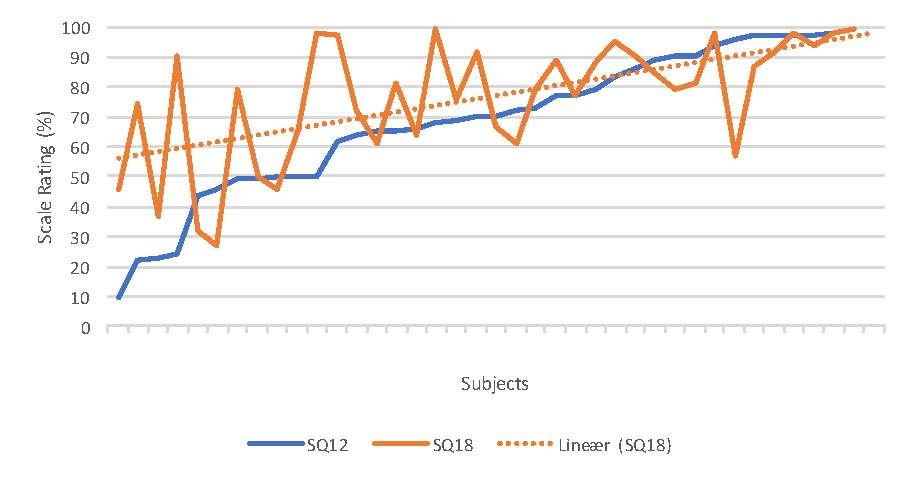
\includegraphics[width = 0.49\textwidth]{Figure/SQ12+SQ18}
	\setlength\abovecaptionskip{-1.2\baselineskip} 
	\caption{Comparison between ratings on SQ12 and SQ18 based on 41 subjects. Two were removed due to incomplete datasets.}
	\label{fig:SQ12+SQ18}
\end{figure}
\noindent
%
\begin{table}
	\centering
	\caption{Correlations from graphs}
	\label{tab:CorrelationsFromGraphs} 
	\begin{tabular}{ c|c }
		\centering
		Positive correlation & Negative correlation \\ \hline
		SQ04 + SQ09 & SQ02 + SQ09 \\ 
		SQ08 + SQ10 & SQ09 + SQ10 \\ 
		SQ08 + SQ17 & SQ12 + SQ21 \\ 
		SQ10 + SQ13 & SQ13 + SQ21 \\ 
		SQ12 + SQ18 & SQ18 + SQ21	\\	
		SQ18 + SQ20 & 							\\
		SQ20 + SQ22 & 
	\end{tabular}        
\end{table}
\noindent
%

The physical variables can be compared with SQs as well as the demographic parameters in the same manner as comparing SQs with each other. \autoref{fig:HeightSQ6} shows SQ6 compared with the robot's height, which shows that when the robot's height increases the robot is perceived as less annoying. Within subjects' age small tendencies were noted. When comparing SQ6 with age, the younger a person is, the more inclined one is to rate the robot as going too slow. Also, a small negative correlation was noted in relation to how exciting and funny the robot seemed. The older the subjects were, the less exciting and funny they rated the robot. Within height the smaller the robot was the faster and more wild it was rated. This was expected, as the robot is programmed from factory to move more slowly when the height increases and faster when it is low. Additionally it was rated more cute, elegant, and trustworthy, regarding to wayfinding, when it was small.
%
\begin{figure}[H]
	\centering
	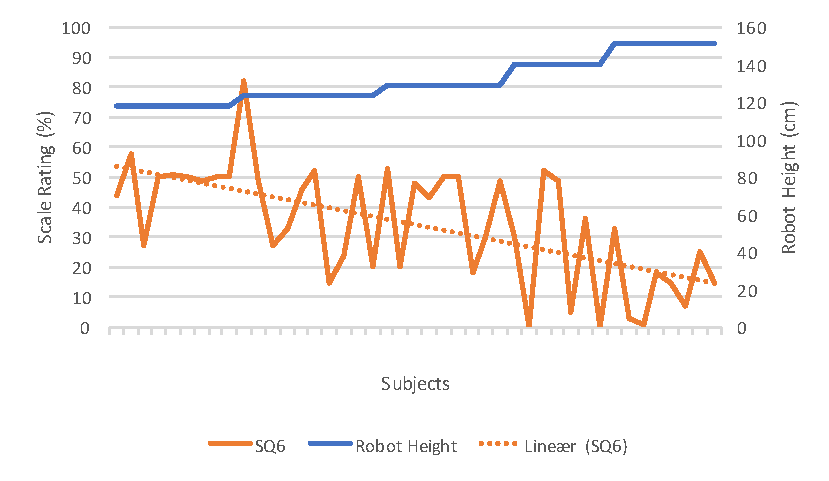
\includegraphics[width = 0.49\textwidth]{Figure/HeightSQ6}
	\setlength\abovecaptionskip{-1.2\baselineskip} 
	\caption{Comparison between the robot's five heights (cm) and ratings on SQ6 based on all subjects.}
	\label{fig:HeightSQ6}
\end{figure}
\noindent
%
